% !TEX encoding = UTF-8 Unicode
% !TEX spellcheck = en-US


% This is the root file of your thesis: thesis.tex
% A line starting with % is a comment. In some cases, I have included a command preceded by a %. You may activate the command by removing the %.

%%===================================
\documentclass[12pt]{report}
\usepackage{ramsstyle}
%%===================================
%Write the various parts of your thesis as separate files and include them into the main file by the command \include{name of included file}. When you compile the LaTeX file, you may choose which subfiles to include by the command

%\includeonly{chapter01,chapter02}

%%===================================
\begin{document}
% !TEX encoding = UTF-8 Unicode
%!TEX root = thesis.tex
% !TEX spellcheck = en-US

%This is the Titlepage
%%=========================================
\thispagestyle{empty}

\includegraphics[scale=1.1]{fig/NTNU}
\mbox{}\\[6pc]
\begin{center}
\Huge{Specification and First Prototype of Simulated Environment for Autonomous USV}\\[2pc]

\Large{Kjetil Save Børs-Lind}\\[1pc]
\large{August 2016}\\[2pc]

TTK4550 - Specialization Project\\
Department of Engineering Cybernetics\\
Norwegian University of Science and Technology
\end{center}
\vfill

\noindent Supervisor: Morten Breivik, ITK

\noindent Co-supervisor: Rein Anders Apeland, Kongsberg Maritime


 % This is the titlepage
\setcounter{page}{0}
\pagenumbering{roman}
% !TEX encoding = UTF-8 Unicode
%!TEX root = thesis.tex
% !TEX spellcheck = en-US
%%=========================================
\addcontentsline{toc}{section}{Preface}
\section*{Preface}
Some preface.\\[2cm]

\begin{center}
Trondheim, 2012-12-16\\[1pc]
(Your signature)\\[1pc]
Ola Nordmann
\end{center}
% !TEX encoding = UTF-8 Unicode
%!TEX root = thesis.tex
% !TEX spellcheck = en-US
%%=========================================
\addcontentsline{toc}{section}{Acknowledgment}
\section*{Acknowledgment}
I would like to thank the following persons for their great help during \ldots

If the project has been carried out in cooperation with an external partner (e.g., a company), you should acknowledge the contribution and give thanks to the involved persons.

You should also acknowledge the contributions made by your supervisor(s).

\begin{flushright}
O.N.\\[1pc]
(Your initials)
\end{flushright}
% !TEX encoding = UTF-8 Unicode
%!TEX root = thesis.tex
% !TEX spellcheck = en-US
%%=========================================
\addcontentsline{toc}{section}{Summary and Conclusions}
\section*{Summary and Conclusions}
Here you give a summary of your your work and your results. This is like a management summary and should be written in a clear and easy language, without many difficult terms and without abbreviations. Everything you present here must be treated in more detail in the main report. You should not give any references to the report in the summary -- just explain what you have done and what you have found out. The Summary and Conclusions should be no more than two pages.

You may assume that you have got three minutes to present to the Rector of NTNU  what you have done and what you have found out as part of your thesis. (He is an intelligent person, but does not know much about your field of expertise.)
\tableofcontents
\setcounter{page}{0}
\pagenumbering{arabic}
% !TEX encoding = UTF-8 Unicode
%!TEX root = thesis.tex
% !TEX spellcheck = en-US
%%=========================================
\chapter{Introduction}
The first chapter of a well-structured thesis is always an introduction, setting the scene with background, problem description, objectives, limitations, and then looking ahead to summarize what is in the rest of the report. This is the part that readers look at first---\emph{so make sure it hooks them!}

%%=========================================
\section{Background}
In this section, you should present the problem that you are going to investigate or analyze; why this problem is of interest; what has, so far, been done to solve the problem, and which parts of the problem that remain.

{\color{red}Below, I have set up some headings (subsection titles) without a number. These are included to help you remember to cover the related issues. The headings should be removed in your final print.}
%%=========================================
\subsection*{Problem Formulation}
You should define your problem in a clear an unambiguous way and explain why this is a problem, why it is of interest---and to whom. It is also important to delimit the problem area.
%%=========================================
\subsection*{Literature Survey}
You should here present the main books and articles that treat problems that are similar to what  you are studying. If you,  later in your thesis, describe the ``state of the art'' -- with a detailed literature survey, you may just give a very brief survey here (approx. a quarter of a page). If this is the only literature survey, you need to go into more details. An objective of the literature survey is to show the reader that you are familiar with the main literature within your field of research -- so that you do not ``reinvent the wheel.''


References to literature can be given in two different ways:
\begin{itemize}
\item As an \emph{explicit} reference: It is shown by \citet{lundteigen08} and partly also by \citet{rausand14}  that \ldots.
\item As an \emph{implicit} reference: It is shown \citep[e.g., see][Chap. 4]{rausand04} that \ldots.
\end{itemize}
In the example above, we have used ``author-year'' references, which is the preferred format. 
\begin{remark}
Following agreement with your supervisor, you may also refer by numbers, for example,  [1]. To do this, open the file \texttt{ramsstyle.sty} and  comment out (by \%) the command \texttt{$\backslash$usepackage\{natbib\}} and un-comment the corresponding command \texttt{$\backslash$usepackage[numbers]\{natbib\}}.\footnote{Notice the strange way we have to write the ``backslash'' in the text. This is because the ``backslash'' is a command in \LaTeX.}
\end{remark}
 You may include a link to the Internet in the text or in a footnote by using a command like: \url{http://www.ntnu.edu/ross}. 

When you refer to the scientific literature, you should always write in \emph{present} tense. Example: \citet{rausand04} show that \ldots.

\begin{remark}
Hyperlinks are included by the command \texttt{$\backslash$usepackage\{hyperref}\} in \texttt{ramsstyle.sty}. If you feel that the hyperlinks are disturbing when you enter the text, or want to avoid the hyperlinks in printed text, you may either comment out or edit this command in \texttt{ramsstyle.sty}.
\end{remark}
%%=========================================
\subsection*{What Remains to be Done?}
After you have defined and delimited your problem -- and presented the relevant results found in the literature within this field, you should sum up which parts of the problem that remain to be solved.
%%=========================================
\section{Objectives}
The main objectives of this Master's project are
\begin{enumerate}
\item This is the first objective
\item This is the second objective
\item This is the third objective
\item More objectives
\end{enumerate}

The objectives shall be written as \emph{fundamental objectives} telling what to do and not \emph{means objectives} telling how to do it.

All objectives shall be stated such that we, after having read the thesis, can see whether or not you have met the objective. ``To become familiar with \ldots'' is therefore not a suitable objective.

%%=========================================
\section{Limitations}
In this section you describe the limitations of your study. These may be related to the study object (physical limitations, operational limitations), to the environmental and operational conditions, to the thoroughness of the analysis, and so on.
%%=========================================
\section{Approach}
Here you should describe the (scientific) approach that you will use to solve the problem and meet your objectives. You should specify the approach for each objective.

If there are any ethical problems related to your approach, these should be highlighted and discussed.
%%=========================================
\section{Structure of the Report}
The rest of the report is organized as follows. Chapter 2 gives an introduction to \ldots

\begin{remark}
Notice that chapter and section headings shall be written in lowercase, but that all main words should start with a capital letter.
\end{remark}


The report should be no longer than \underline{60 pages} in this format (+ the CV).
% !TEX encoding = UTF-8 Unicode
%!TEX root = thesis.tex
% !TEX spellcheck = en-US
%%=========================================
\chapter{Existing Solutions}


\section{CyberSea Simulator}
The CyberSea Simulator developed by Marine Cybernetics is a simulator for HIL testing of Dynamic Positioning (DP) systems.

Key points from [\cite{HILtestingDP}]:
\begin{itemize}
\item Capabilities for data logging and real-time presentation of results
\item Emphasis on vessel dynamics and accurate simulation of vessel motion at low speed ( < 3kts, wave, wind and current loads (of course, because of DP) in six degrees of freedom "using a nonlinear rigid-body model of the vessel".
\item Several options for interface between HIL Simulator and Computer Control System ("Analog, digital, serial/NMEA protocol", normal network protocol or "dedicated test I/O built into the DP computer system").
\item Generation of realistic signals from all the common sensors and position reference systems (such as "Gyro-compasses, VRUs, wind sensors, thruster feedback [...], power feedback from thrusters, switchboard and generator sets") used in modern DP technology "contaminated with typical noise levels".
\item Advanced generation of GNSS signals with possibility of simulating a broad specter of common failure modes.
\end{itemize}


\section{MSS (Fossen)}

\section{MCSim (Marine Cybernetics)}

\section{Gazebo (ROS)}
% !TEX encoding = UTF-8 Unicode
%!TEX root = thesis.tex
% !TEX spellcheck = en-US
%%=========================================
\chapter[Summary]{Summary and Recommendations for Further Work}

%%=========================================
\section{Summary and Conclusions}

%%=========================================
\section{Discussion}
%%=========================================
\section{Recommendations for Further Work}

% Include more chapters as required.
%%=========================================
\appendix
% !TEX encoding = UTF-8 Unicode
%!TEX root = thesis.tex
% !TEX spellcheck = en-US
%%=========================================

\chapter{Acronyms}
\begin{description}
\item[FTA] Fault tree analysis
\item[MTTF] Mean time to failure
\item[RAMS] Reliability, availability, maintainability, and safety
\end{description}
% !TEX encoding = UTF-8 Unicode
%!TEX root = thesis.tex
% !TEX spellcheck = en-US
%%=========================================

\chapter{Additional Information}
This is an example of an Appendix. You can write an Appendix in the same way as a chapter, with sections, subsections, and so on.

%%=========================================
\section{Introduction}

%%=========================================
\subsection{More Details}
% Include more appendices as required.
%%=========================================
\bibliographystyle{apa}
\addcontentsline{toc}{chapter}{\bibname}
\bibliography{refs}  
%%=========================================
% !TEX encoding = UTF-8 Unicode
%!TEX root = thesis.tex
% !TEX spellcheck = en-US

%This is the Curriculum Vitae
%%=========================================
\addcontentsline{toc}{chapter}{Curriculum Vitae}
\chapter*{Curriculum Vitae}
\hrule
\begin{minipage}[t]{0.65\linewidth}
\begin{tabular}{ll}
Name: & \textbf{Your Name}\\
Gender: & Female\\
Date of birth: & 1. January 1995\\
Address: & Nordre gate 1, N--7005 Trondheim \\
Home address: & King's road 1, 4590 Vladivostok, Senegal\\
Nationality:    & English \\
Email (1): & your.name@stud.ntnu.no\\
Email (2): & yourname@gmail.com\\
Telephone: & +47 12345678\\
\end{tabular} 
\end{minipage}\hfill
\begin{minipage}[t]{0.25\linewidth}
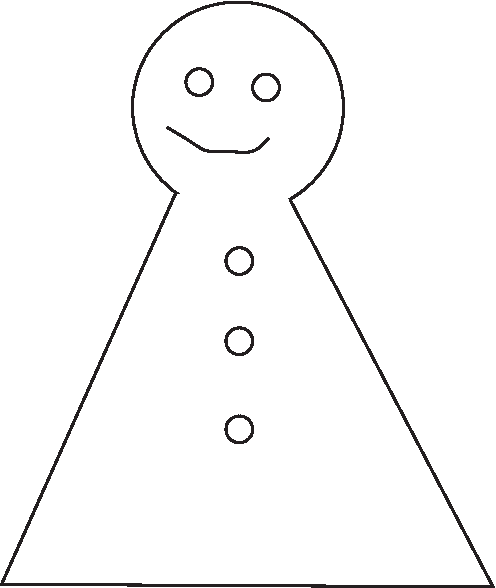
\includegraphics[scale=0.3]{fig/me}\\[1pc] Your picture
\end{minipage}
\hrule

%%=========================================
\section*{Language Skills}
Describe which languages you speak and/or write. Specify your skills in each language.

%%=========================================
\section*{Education}
\begin{itemize}
\item School 1
\item School 2
\item School 3
\end{itemize}

%%=========================================
\section*{Computer Skills}
\begin{itemize}
\item Program 1
\item Program 2
\item Program 3
\end{itemize}

%%=========================================
\section*{Experience}
\begin{itemize}
\item Job 1
\item Job 2
\item Job 3
\end{itemize}

%%=========================================
\section*{Hobbies and Other Activities}         % Your curriculum Vitae     
%%=============================================

\end{document}
